\documentclass[12pt,fleqn]{article}\usepackage{../../common}
\begin{document}
Log Lineer Modeller ve Koşulsal Rasgele Alanlar (Log Linear Models and Conditional Random Fields -CRF-)

Charles Elkan ders notları

Elkan'ın yapay öğrenim konusuna bakışı ilginç, ona göre yapay öğrenim
bir bilgisayar bilim (computer science) konusudur, mesela altta işlenen
maksimum olurluk bilgisayar bilimdir. 

Koşulsal Olurluk (Conditional Likelihood)

Diyelim ki elimizde eğitim verisi olarak ikili $< x,y >$ veri noktaları
var. O zaman $y$'nin $x$'e koşulsal olarak bağlı (conditional on) bir
dağılımı olduğunu söyleyebiliriz. 

$$ y \sim f(x;\theta) $$

Yani her $x$ için farklı bir $y$ dağılımı ortaya çıkabilir. Ve tüm bu
farklı dağılımların ortak noktası $\theta$ parametresidir. Koşulsal
olasılık yani şöyle yazılabilir, 

$$ P(Y=y | X=x;\theta) $$

Üsttekiler $Y$ için bir model ortaya koydu, peki elimizde $X$'in dağılımı
için bir olasılık modelimiz var mı? Cevap hayır. Niye? Düşünelim, $p(y,x)$
nedir ?

$$ p(x,y) = p(x)p(y|x) $$

Üstte $p(y|x)$'i tanımlayacak ($\theta$ üzerinden) bir olasılık demeti /
ailesi tanımladık, fakat elimizde $p(x)$ dağılımını verecek bir model
yok, o zaman $p(x,y)$'yi tanımlayacak bir model de yok.

Fakat bu dünyanın sonu değil. Belki de Yapay Öğrenim (machine learning)
branşının bir sloganı şu olmalı: ``Öğrenmen gerekmeyen şeyi
öğrenme''. Üstteki örnekte $p(y|x)$'i öğrenebiliriz, ama $p(x)$'i illa
öğrenmemiz gerekir mi?

Sınıflayıcı (classifier) ve denetimli (supervised) öğrenim durumunu
düşünürsek, bize eğitim amaçlı olarak $< x,y >$ ikili veri noktaları
sağlanacak. $x$ kaynak veri, $y$ tahmin edilecek (ya da başta eğitim hedefi
olan) etiket olacak. $y$ için bir model ortaya çıkartıyoruz, çünkü test
zamanında $y$ olmayacak, fakat $x$ hep olacak. Yani $y$'nin modellenmesi
mecburi, çünkü ``genelleyerek'' onun ne olduğunu bulacağız, ama $x$ hep
verili.

Koşulsal Olurluk Maksimum Olurluk Prensibi

Eğitim verisi $< x_1,y_1 >,...,< x_n,y_n >$ için, $\theta$'yi şöyle seç

$$ \hat{\theta} =  \arg\max_{\theta} \prod _{i=1}^{n} p(y_i | x_i;\theta) $$

Normal maksimum olurlukta bilindiği gibi olasılıkların çarpımı maksimize
edilir, burada maksimize ettiğimiz ``koşulsal'' olasılıkların çarpımı. 

Burada önemli bir soru şu: bildiğimiz gibi maksimum olurluk hesabı her veri
noktasının bir diğerinden bağımsız olduğunu farzeder [çünkü her olurluk
hesabını bir diğer ile çarpıyoruz, başka ek çarpım, toplama, vs
yapmıyoruz], bu faraziye doğru bir faraziye midir? Bu soru ve ona verilecek
cevap çok önemli. Evet, eğer eğitim noktaları birbirinden bağımsız değilse
maksimum olurluk kullanmamalıyız. Bağımsızlığı da iyi tanımlamak gerekiyor
tabii, eğer üstteki durumda $x_i$ {\em verildikten sonra} $y_i$'ların
birbirinden bağımsız olması yeterli.

Bu model klasik İstatistik'te çokça kullanılan bir yaklaşımdır, hatta
lineer regresyon'un temeli üstteki faraziyedir. 

$$ y = \alpha + \bar{\beta}\bar{x} + N(0,\sigma^2) $$

Bu standart lineer regresyon modeli, ve bu modelde her $y$ ona tekabül eden
$x$'e bağlı, bu sayede $x$'ler biliniyorsa $y$'ler birbirinden koşulsal
olarak bağımsız hale geliyor, böylece $x$'ler birbirine bağımlı olsa bile
$\alpha$ ve $\beta$'nin bulunması mümkün oluyor. 

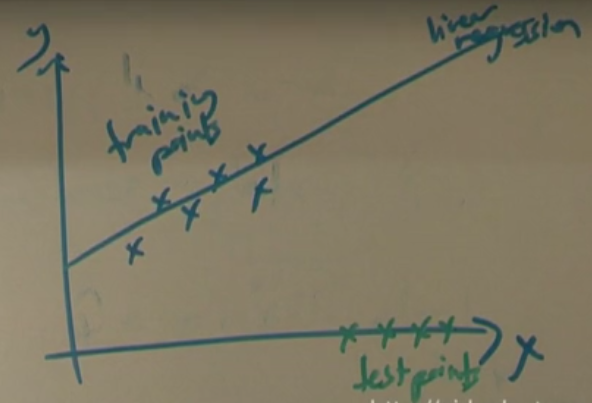
\includegraphics[height=4cm]{crf_1.png}

Üstteki resimde eğitim noktaları (training points) mavi olsun, test noktaları
yeşil olsun (hemen altında). Bazı Yapay Öğrenim yaklaşımları diyebilir ki eğitim
$x$'lerinin dağılımı test $x$'lerinin dağılımından farklı, bu veri seti
öğrenilemez (yani genellenemez, modellenemez). Fakat klasik İstatistik buna
bakar ve der ki $x$'lerin verildiği durumda $y$'ler bağımsızdır, bu şekilde bir
koşulsal model öğrenilebilir.

Lojistik Regresyon aynı şekilde işler (lojistik regresyon, log lineer
modellerin özel bir halidir, CRF'ler aynı şekilde). Burada
da öğrenilen bir

$$ p = p(y | x;\alpha,\beta) $$

modeli vardır ve $y$ değerleri sadece 0 ve 1 olabilir. Tahmin edilen
olasılık ise $y$'nin 1 olma olasılığıdır. Bu model Rasgele Gradyan Çıkışı
ile eğitilir [detaylar için bkz {\em Lojistik Regresyon} notları].

$$ log \frac{p}{1-p} = \alpha + \sum_j \beta_j x_j $$

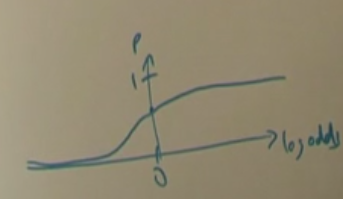
\includegraphics[height=4cm]{crf_2.png}

$p$ log şansının monotonik bir fonksiyonudur, ve ters yönden bakarsak, log
şans $p$'nin monotonik bir fonksiyonudur. Yani lineer bir fonksiyon (sağ
taraf) ne kadar büyürse, olasılık / log şans o kadar büyüyecektir. Bu
büyüme durumu mesela $\beta_j$ katsayısını veri analizi bağlamında
yorumlanabilir hale getirir. Diyelim ki $\beta_4$ katsayısı pozitif, o
zaman diğer tüm şartların eşit olduğu durumda (with all else being equal)
$x_4$ ne kadar buyurse 1 olma olasılığı o kadar artar.

Lojistik modellerin önemli bazı avantajları var, ki bu avantajlar log
lineer modellere de sirayet ediyor (bu iyi). 

1) Değişkenler arası ilinti (correlation) probleme yol açmaz: Bu fayda aslında
daha önce belirttiğimiz $x$'lerin birbirine bağımlı olabilmesi ile
alakalı. Bağımsızlık önşartı aranmadığı için istediğimiz kadar $x$'i problemin
üzerine atabiliriz, eğitici algoritma bunlardan çıkartabildiği kadar iyi bir
model bulacaktır.

Kıyasla mesela Naive Bayes böyle değildir, eğer bir NB sınıflayıcısını
eğitiyorsak, ve öğelerin (feature) arasında ilinti var ise, sınıflayıcının
doğrulugu (accuracy) azalabilir.

2) LR ile ``1 olma olasılığını'', yani ``bir sayısal skoru'', elde
ediyoruz, bu sadece 1/0 değerinden daha fazla bir bilgi demektir.

3) Bu skor, anlamı olan bir olasılıksal değerdir: Sonuçta SVM
sınıflayıcıları da $-\infty$ ve $+\infty$ arasında değerler döndürürler, ve
bu değerler sıralama (ranking) amaçlı kullanılabilir, fakat olasılık
matematiği açısından anlamı olan bir değerin olması bundan bile
iyidir. Naive Bayes 0 ve 1 arasında değer döndürebilir, fakat bu değerlerin
de olasılıksal olarak aslında anlamı yoktur, pratikte görüldü ki bu
değerler çok uç noktalarda, ya sıfıra çok yakın, ya bire çok
yakın. Literatürde NB skorlarının ``iyi kalibre edilmiş olmadığı''
söylenir.

$X_1,...,X_n$ test örnekleri ve tahmin edilen olasılıklar $P(Y=1 | x_i) = v_i$ 
olsun. Diyelim ki $s = \sum_i v_i$ ve $t$ sayısı $1,..,n$ tane öğenin
içinden $y = 1$ değerini taşıyan öğelerin sayısı olsun. Örnek, elimizde 100
tane eğitim noktası var, bunların 60'ı 1 değerinde. Bu durumda $s$ yaklaşık
60 olacaktır (rasgele gürültüyü hesaba katarsak tabii), yani  $E[t] = s$ 
denebilecektir ve bu sadece eğer olasılıklar iyi kalibre edilmişse
söylenebilir.

4) Dengesiz eğitim verisi kullanılabilir: pek çok eğitim setinde mesela 1
değeri taşıyan değerleri 0 değeri taşıyanlardan çok daha fazla. Lojistik
regresyon bu tür veriyle rahatça çalışabilir.
 
Ders 3

Lojistik regresyon için log olurluğun (LCL) türevini almak lazım. Önce
basitleştirme amaçlı $\alpha = \beta_o$, ve $x_0 = 1$. O zaman log şansın
eski hali (altta eşitliğin sol tarafı) şöyle yazılabilir (sağ taraf), daha
derli toplu bir formül olur,

$$ \alpha + \sum_j \beta_j x_j  = \sum_{j=0}^{d} \beta_j x_j $$ 

Bulmak istediğim her $j$ için $\frac{d}{d\beta_j} LCL$ lazım

$$ 
\frac{d}{d\beta_j} LCL = 
\sum _{i:y_i=1} \frac{d}{d\beta_j} \log p(1|..)
+ \sum _{i:y_i=0} \frac{d}{d\beta_j} \log p(0|..)
\mlabel{3}
$$

Eğer üstteki bir bölümü $p$ diğerine $1-p$ dersem, yani şöyle

$$ 
= \sum _{i:y_i=1} \frac{d}{d\beta_j} \underbrace{\log p(1|..)}_{p}
+ \sum _{i:y_i=0} \frac{d}{d\beta_j} \underbrace{\log p(0|..)}_{1-p}
$$

O zaman 


$$ 
= \sum _{i:y_i=1} \frac{d}{d\beta_j}\log p
+ \sum _{i:y_i=0} \frac{d}{d\beta_j} \log (1-p)
$$

Biliyoruz ki

$$ 
\frac{d}{d\beta_j}\log p = \frac{1}{p}\frac{d}{d\beta_j} p
\mlabel{1}
$$

$$ 
\frac{d}{d\beta_j}\log (1-p) = \frac{1}{1-p}(-1)\frac{d}{d\beta_j} p
\mlabel{2}
$$

Üstteki son iki formülün her ikisinde de $d/d\beta_j p$ kısmı olduğuna dikkat.

Notasyon

$$ e = \exp \big[ - \sum_{j=0}^n \beta_jx_j \big] $$

$$ p = \frac{ 1}{1+e} $$

$$ 1-p = \frac{ 1+e-1}{1+e} = \frac{ e}{1+e} $$

Şimdi  $d/d\beta_j p$'e dönelim, ve $p$'nin üstteki gibi olduğundan
hareketle,

$$ \frac{ d}{d\beta_j}p = (-1)(1+e)^{-2} \frac{ d}{d\beta_j}e $$

$$ = (-1)(1+e)^{-2} (e) \frac{ d}{d\beta_j}(x_j) $$

$$ = \frac{ 1}{1+e} \frac{ e}{1+e}x_j = p(1-p)x_j$$

Son ifade kodlama için oldukça uygun, $d/d\beta_j p$ hesabını yine içinde
$p$ içeren bir ifadeye bağladık, ayrıca türev $x_j$ ile orantılı. 

Bu hesapla aslında (1) içindeki $d/d\beta_j p$ kısmını hesaplamış
olduk. Eğer yerine koyarsak, 

$$ 
\frac{d}{d\beta_j}\log p = \frac{1}{p}p(1-p)x_j 
$$

$p$'ler iptal olur

$$ 
= (1-p)x_j 
$$

Aynı şekilde (2) için 

$$ 
\frac{d}{d\beta_j}\log (1-p) = \frac{1}{1-p}(-1) p(1-p)x_j 
$$

$$ 
 =  -px_j 
$$

Üstteki türevler tek bir eğitim veri noktası için. Tüm eğitim veri setinin
türevi her noktanın türevlerinin toplamı olacak, (3)'de görüldüğü gibi.

$$ \frac{d}{d\beta_j} LCL = 
\sum _{i: y_i = 1} (1-p_i)x_{ij} + 
\sum _{i: y_i = 0} -p_i x_{ij}  
\mlabel{4}
$$

$x_{ij}$ notasyonunda $j$, $j$'inci öğe / özellik anlamına geliyor. Şimdi 
notasyonel bir numara kullanacağım, 

$$ = \sum _{tum \ i} (y_i - p_i)x_{ij} $$

Bunu niye yaptım? (4) formülünde eşitliğin sağ tarafı, birinci terim içinde
1 sayısı var, sonraki terimde 1 yok. Eğer 1 olup olmaması yerine $y_i$
kullanırsam, ki zaten 1'in olup olmaması $y_i$'nin 1 olup olmamasına bağlı,
tek bir terimde işi halledebilirim. $y_i=1$ olduğu zaman üstteki ifade
$1-p_i$ olacaktır, olmadığı zaman $-p_i$ olacaktır. 

Eriştiğimiz sonucu analiz etmemiz gerekirse, nihai formül gayet basit ve
temiz çıktı. 

[24:10] kalibrasyonla alakalı bir yorum

Rasgele Gradyan Çıkışı (Stochastic Gradient Ascent)

Fikir: türevi eğitim noktası basına hesapla, ve modeli hemen güncelle. 

Eğitim noktaları $< x,y >$ olarak gelsinler. Her nokta için, ve her $\beta_j$
için

$$ \frac{d}{d\beta_j}p(y|x;\beta) = g_j$$ hesapla. 

$$ \beta_j := \beta_j + \alpha g_j $$

Gradyanın ne olduğunu hatırlayalım, bir fonksiyonun maksimumuna ``doğru''
olan bir gidiş yönünü gösterir, ve bu gidiş yönü o fonksiyonu oluşturan
değişkenlerin (parçalı türevleri) üzerinden belirtilir. O zaman elimizdeki
gradyan o iç değişkenlerin maksimum yöndeki değişim şeklini bize tarif
eder. 

Algoritmanın tamamı: alttaki formül için

$$ \frac{d}{d\beta_j}p(y|\bar{x};\bar{\beta}) = (y-p)x_j $$

Her $x$ için

- O anki modele göre $p$'yi hesapla

- Her $j = 0,..,d$ için

\ \ \ - $ \beta_j := \beta_j + \alpha \underbrace{ (y-p) x_j}_{\textrm{kısmi türev}} $ hesapla
  
Peki metotun ismindeki ``rasgele (stochastic)'' tanımı nereden geliyor? İyi
bir soru bu çünkü metotta rasgele sayı üretimi gibi şeyler
görmüyoruz. Cevap, metot yine de rasgele, çünkü her noktayı ayrı ayrı
işliyoruz, ve bu noktaların eğitim algoritmasını gelişi bir nevi ``veriyi
örneklemek'' gibi sanki, ek olarak veriyi eğitime almadan önce rasgele
şekilde karıştırmak ta iyi olabilir. 

Bazı Tavsiyeler (Heuristics)

1) Her özellik (feature) $x_j$'i ölçeklemek, yani aynı ortalama (mean) ve
varyansa sahip olacak şekilde tekrar ayarlamak. Yani mesela 0 ile 100
arasında olabilecek ``yaş'' gibi bir özelliği, 0 ve 1 arasında değişen
özellikler ile aynı ortalama ve varyansa sahip olacak şekilde
ayarlamak. Bunun sebebi güncelleme hesabındaki $\lambda$'nin tek bir sabit
olması, ve bu sabit her $j$ için aynıdır, o sebeple $\lambda$'nin her öğeye
``aynı şekilde'' uygulanabilmesi için öğelerin birbirine yakın olması
iyidir. Ek olarak, genellikle eğitim verisinde 0 ile 1 arasında ikisel
türden öğeler vardır, o sebeple bu şekilde olmayan diğer ögeleri 0 ve 1
arasında çekmek daha uygun ve kolay olur.

2) Veriyi rasgele şekilde sıralamak. Terminoloji: eğitim veri seti
üzerinden bir geçiş yapmak bir ``çağ'' (epoch) olarak bilinir. 

3) $\lambda$'yi deneme / yanılma yöntemi ile bulun (bu sabiti bulmanın
sistemik bir yöntemi yok). Belki verinin içinden alınan daha ufak bir
örneklem üzerinde bu deneme / yanılma işlemi yapılabilir.

4) Deneme yanılma işlemini şöyle yapabilirsiniz: büyük bir $\lambda$ ile
ise başlarsınız, ve her çağda $\lambda$ değerini azaltabilirsiniz (mesela
her çağ sonunda $1/2$ ile çarparak).

Ders 4

Log Lineer Modeller

Bu modeller lojistik regresyonun yapıya sahip (structured) girdiler ve
çıktılar için genellenmiş halidir. Lojistik regresyonda girdi $\bar{x} \in
\mathbb{R}^d$ ve çıktı $y \in {0,1}$ idi, yani çıktı ikiseldi. Fakat biz bundan 
daha genel yapay öğrenim problemlerini çözmek istiyoruz, yani 
istediğimiz $x \in \mathbb{X}$, ki $\mathbb{X}$ herhangi bir 
uzay olabilmeli, ve $y \in \mathbb{Y}$ ki $\mathbb{Y}$ aynı şekilde
herhangi  bir uzay olabilmeli. 

Mesela $x$ bir cümle olabilmeli, diyelim ki $x$ = ``he sat on the mat'',
tercümesi ``adam paspasın üzerinde oturdu''. Buna karşılık olan $y$ ise
mesela şöyle olabilmeli, $y$ = ``pronoun verb article noun'', yani her
kelimenin hangi gramer ögesi olduğunu gösteren bir ibare. Mesela ``sat''
yani oturmak, bir fiil (verb), ``mat'' paspas, bir isim (noun), ve $y$
içinde gelen eğitim verisinde bunlar olabilmeli (üstteki örnekte ikinci
öğe), sadece 0/1 değerleri değil.

Bu tabii ki denetimli bir eğitim şekli olacak. Fakat dikkat bazı yapay
öğrenim uygulamalarında ``çok sınıftan gelen'' ama tek bir değer vardır,
mesela $y \in {1,2,3}$ olabilir, 3 sınıflı bir çıktı yani. Bazen çıktı
gerçek sayı (real number) olabilir, ama yine de tek bir $y$ değeri
vardır. Üstteki durum böyle değildir. Potansiyel olarak $y$'nin büyüklüğü
$x$ ile birebir aynı bile olmayabilir. Bu tür bir karışık eşlemeden
bahsediyoruz.  Tek sınırlamamız $\mathbb{Y}$'nin sonlu (finite) olması.

Model şöyle (notasyonu biraz değiştirdik, $\beta$ yerine $w$ kullanıyoruz
mesela, $w$ modelin ``ağırlıklarını (weights)'' temsil ediyor. 

$$ p(y|x;w) = 
\frac{\exp \big[ \sum_{j} w_j F_j (x,y) \big]}{Z(x,w)}
$$

Yakından bakarsak model LR modeline benziyor. Bir lineer fonksiyonun
$\exp$'sı alınıyor ve bu değer olasılık hesabında kullanılıyor. İleride
zaten göreceğiz ki LR üstteki yaklaşımın bir ``özel durumu'', yani üstteki
model daha genel bir tanım. 

Aklımıza birçok soru geliyor herhalde, mesela ``$Z$ nedir?'' ya da ``$F_j$
nasıl hesaplanır?'' gibi. $Z$ şöyle tanımlanır

$$ Z(x,w) = \sum_{y'} \exp \big[ \sum_j w_j F_j(x,y') \big] $$

Tüm $y'$'lere bakılıyor, yani tüm mümkün $\mathbb{Y}$ değerleri teker teker
$y'$ üzerinden toplamda kullanılıyor. $\mathbb{Y}$'nin sonlu olma
faraziyesi burada önemli hale geliyor, toplamı sonsuz bir küme üzerinden
yapamayız. 

$Z$ normalizasyon için kullanılıyor, çünkü olasılık teorisinde eğer
elimizde çoklu bir hedef var ise, bu hedeflere olan olasılık değerlerinin
toplamı 1 olmalıdır. $Z$ işte bunu garantiler, bu sebeple bölen
(denominator) bölümün (nominator) toplamı olmalıdır. 

Her $F_j(x,y)$ bir özellik fonksiyonudur (feature function). Niye? Çünkü
elimdeki $x$'ler illa bir vektör olmayabilir, yani $x_j$ ``vektörünü'' alıp
$w_j$ ``vektörü'' ile çarpamam, bu sebeple önce bir fonksiyon ile bir
sayısal (numerical) değer üretmem gerekiyor. Küme olarak

$$ F_J: \mathbb{X} \times \mathbb{Y} \to \mathbb{R} $$

Eğer $ F_j(x,y) > 0 $ ve $w_i > 0$ ise, o zaman $F_j(x,y) = 0$'a kıyasla
$p(y|x;w)$ artar. Sezgisel olarak tarif edersek özellik fonksiyonun (OF)
söylediği şudur, eğer ağırlık pozitif ise OF'in değeri ne
kadar buyurse elimizdeki $y$, $x$ ile o kadar ``uyumludur'' (tabii ki belli
bir özellik yani $j$ için). Negatif ilinti bunun tam tersi olurdu. 

Eğitim $w_j$ ağırlıklarını bulmamızı sağlar. $F$ önceden tanımlıdır (yani
eğitime bile başlamadan önce), bu fonksiyonun ne olacağı
``seçilir''. Seçilirken tabii ki $x,y$ arasındaki ilintiye göre fazla / az
sonuç geri getirebilecek şekilde seçilmelidir. 

Kelime örneğine geri dönersek, bir $F$ şöyle olabilir, 

$ F_{15}(x,y) =$ ``eğer ikinci kelimenin baş harfi büyük ve ikinci etiket
isim (noun)''. OF'ler reel değerlidir. Bunun özel durumu 0/1 değeri veren
OF'lerdir. Biraz önceki örnek mesela 0/1 döndürüyor.

Ya da $F_{14}(x,y)$ diyelim ki şöyle ``ilk kelimenin baş harfi büyük, ve
ilk etiket bir isim''. Tahmin edebiliriz ki eğitim setimizde ilk
kelimesinin baş harfi büyük {\em olan} ama o kelimesi isim olmayan pek çok
örnek olacaktır. Bu durumda $w_{14}$ küçük olur. 

Dediğimiz gibi $F$ reel değeri olabilir, mesela

$$ F_{16}(x,y) = length(y) - length(x) $$

yani bu fonksiyonda $x$'nin uzunluğunu $y$'nin uzunluğundan
çıkartıyoruz. Bu ne işe yarar? Diyelim ki otomatik tercüme yapması için bir
yapay öğrenim programı yazıyoruz, $x,y$ eğitim noktaları birbirinin
tercümesi olan İngilizce/Fransızca cümleler. Çoğunlukla Fransızca cümleler
tekabül ettikleri İngilizce cümlelerden çok daha uzun oluyorlar, yani
üstteki çıkarma çoğunlukla pozitif sonuç verecek. Değişik bir açıdan
bakarsak, pozitif bir sonuç, bir tercümenin doğru olduğu yönünde bir işaret
olarak kabul edilebilir, ve üstteki OF üzerinden eğitim algoritması bunu
kullanır. Eğitim sonrası $w_{16}$ pozitif bir ağırlık alacaktır.

Bir log lineer modelde (buna CRF'ler de dahil) ilk yapılan iş probleminiz
için önemli olan OF'leri ortaya çıkartmak.

$F$ tanımlamanın değişik bir başka yolu:

$a(x)$ bir fonksiyon olsun. Her $v \in \mathbb{Y}$ için

$$ F_j(x,y) = a(x) I(y=v)$$

tanımlayalım. 

$$ p(y|x;w) = \frac{\exp \sum_j w_j F_j (x,y)}{Z} $$

Şimdi lineer zincirli CRF konusuna bakalım. Yine $x \in \mathbb{X}$ ve $y
\in \mathbb{Y}$.  $x$ bir girdi zinciri, $y$ bir çıktı zinciri ve en basit
durumda $x$ ile aynı uzunlukta. Konuşma bölümlerini etiketlemek bu
kategoriye dahil, ama bir diğer uygulama kelimeyi arasına eksi işaretleri
koyarak bölme (hyphenation). 

Mesela girdi $x=$''beloved'', çıktı $y=$''00100000'' çünkü bu kelime
``be-loved'' olarak bölünür. 

Bu uygulama için bir OF 

$$ F_j(x,y) = \frac{\textrm{kaç  tane 1 var}}{\textrm{x uzunluğu}} $$

$x=$''beloved'', çıktı $y=$''00100000'' için sonuç $1/7$ olurdu.

Lineer zincir CRF için hangi OF'lerin bazı sınırları var. 

$$ F_j (\bar{x},\bar{y}) = \sum_i f_j(y_{i-1}y_i\bar{x} i) $$

ki sembol üzeri düz çizgiyi ($\bar{x}$ gibi) bu sefer bir sıralı veri
temsil etmek için kullanıyorum)

Mesela

$$ f_{18} =   f_j(y_{i-1}y_i\bar{x} i) = " i=2, y_{i-1} = 0, y_i = 1,
x_1x_2 = "as" "$$

Mesela ``async'' kelimesi ``a-sync'' olarak bölünebilir, ve eğitim setinde
``async'' ile ``$y=$01...'' gelirse üstteki OF bu bölünmeyi ödüllendirir /
öğrenir.

Şimdi CRF olmayan bir Lineer Model'e bakalım, 

Mesela çok etiketli denetimli (supervised) öğrenim. ``Çok etiketli'' ne
demektir?  Dikkat, ``çok sınıflı (multi label)'' değil, yani tek öğenin iki
veya daha fazla değer arasından birini seçmesinden bahsetmiyoruz. Birden
fazla etiket alabilmekten bahsediyoruz, mesela bir İnternet sayfası, bir
veya daha fazla kategoriye aynı anda ait olabilir, mesela hem Spor, hem İş
Dünyası. Diyelim ki 10 mümkün etiket var, bir doküman kaç değişik şekilde
etiketlenebilir?

$2^{10} = 1024$ şekilde (bu sayı, hesap bir kümenin kaç değişik şekilde alt
kümesi olabilir hesabını yansıtıyor aynı zamanda, yani sıralama önemli
olmadan belli sayıda öğenin kaç değişik şekilde alt kümeleri olabilir
sorusu). Bu büyük bir rakam. Ve bu kadar çok olasılık var ise, eğitim
verisi tüm kombinasyonlar için örnek veri içermeyebilir. Fakat muhakkak
algoritmamızın bu kombinasyonları tahmin edebilmesini tercih ederiz.

Çözüm? 10 değişik sınıflayıcı kurarark bu problemi çözebiliriz (ayrı ayrı,
tek başına tek sınıfa bakılınca yeterli veri çıkar herhalde), fakat bu
şekilde ``sınıflararası'' ilişkileri yakalayamayız. Log lineer model
yaklaşımında öyle bir ikisel (binary) OF yaratırsınız ki, mesela,

$$F_{19}(x,y) = "Spor \in y, \textrm{İş Dünyası} \in y" $$ 

Dikkat edersek OF sadece $y$'ye bakıyor. Bu OF'yi içeren algoritma
eğitilince üstteki OF için bir pozitif ağırlık öğrenilebilecektir. 

Soru: bir anlamda problemin yerini değiştirmiş olmuyor muyuz? Mesela
üstteki şekilde bu sefer her türlü kombinasyon için OF'mi yaratacağız?
Cevap: eğer sadece ikili eşlere bakıyorsak, kombinasyon hesabı 
$C(10,2) = 45$ sonucunu verir. Bu fena bir sayı değil.

Ayrıca verinin seyrekliği bize hangi kombinasyonların dahil edilip
edilmeyeceği yönünde yardımcı olabilir. 

Soru: çok sınıflı problemler lojistik regresyonu geliştirerek çözülemez mi?
Cevap: böyle bir yaklaşım var, buna multinom lojistik regresyon
deniyor. Fakat bu yaklaşımın log lineer modellerin özel bir hali olduğunu
belirtmek isterim, yani yapay öğrenim dünyasının aktif olarak araştırdığı
alan artık burası, multinom lojistik regresyon aşıldı. Zaten log lineer
modeller ile çok etiketli problemleri de çözebiliyorsunuz.

Ders 5

Soru: biraz önce sadece $y$'ler arasında bir OF tanımlayabildiğimizi
gördük. Peki sadece $x$'ler arasında OF tanımlamak faydalı olur muydu?
Cevap: Formülü tekrar hatırlayalım,

$$ p(y|x;w) = \frac{\exp \sum_j w_j F_j (x,y)}{Z(x,w)} $$

OF'nin görevi hangi $y$'lerin daha yüksek olasılığı olduğunu
belirtmek. Eğer sadece $x$ var ise, bu durumda bölüm ve bölendeki değerler
birbirini iptal ederdi. Her $y$ için aynı $x$ ``katkısı'' olurdu ve bunun
sınıflayıcıya hiçbir faydası olmazdı. 

[8:00-18:00 atlandı]

Çözdüğümüz problemler şu formatta

$$ p(\bar{y}|\bar{x};w) = \frac{\exp \sum_j w_j F_j (\bar{x},y)}{Z(\bar{x},w)} $$

Tahmin etmek için 

$$ \hat{y} = \arg\max_{y}  \exp \sum_j w_j F_j(\bar{x},y)$$
Bir $\bar{y}$ tahmin etmek için bu modellerden birini kullanacaksak, $
p(\bar{y}|\bar{x};w)$ formülüne $\bar{x}$'i koyarız, ve elde edilen
dağılımda hangi $\bar{y}$'nin olasılığı daha yüksekse onu seçeriz. Daha
yüksek olasılığa sahip olan $\bar{y}$, $p(\bar{y}|\bar{x};w)$ formülünde
bölümü daha yüksek olandır. Bölen her $\bar{y}$ için sabit / aynı.

Aslında $\exp$'ye ihtiyaç yok, çünkü $\exp$ monotonik bir fonksiyon, yani
sadece şu kullanılabilir,

$$ \hat{y} = \arg\max_{y}  \sum_j w_j F_j(\bar{x},y)$$

En olası $y$'yi bulmak için $Z$'nin gerekmediğine de dikkat, çünkü bu sabit
tüm seçenekler için aynı.

Burada tahmin etmek bağlamında zor olan şey, en yüksek $y$'yi bulmak
için tüm $y$'lere teker teker bakmaya mecbur olmamız. Bu bakma işlemi
çok zaman alabilir, o zaman bu problemi bir şekilde çözmem lazım. 

Diğer problem, tüm olasılıkların 1'e toplanabilmesini sağlayan normalize
sabitinin hesabı, yani $Z(\bar{x},w) = \sum_{y'}\exp [ \sum_j w_j F_j(\bar{x},\bar{y})]$, 
ki eğer olasılık değeri hesaplayacaksak bu sabit gerekli. 

Yani iki ana problem var, bir de eğitim algoritması var, ki bu aynen
lojistik regresyon örneğinde olduğu gibi rasgele gradyan çıkışı üzerinden
olacak, bu 3 algoritmayı şimdi sunacağız. 

Algoritma 1

Önce,

$$ \hat{y} = \arg\max_{\bar{y}}  \sum_j w_j F_j(\bar{x},\bar{y})$$

Bu hesabı polinom zamanda (polynomial time) yapmak istiyoruz. Tanımı biraz
değiştirelim, 

$$ = \arg\max_{\bar{y}}  \sum_j w_j \sum_i f_j(y_{i-1}y_i \bar{x} i )$$
$j$ tüm özellikler, $i$ $x,y$ ``boyunca'' ilerleyen indisler. Üstteki ibare
tek bir eğitim veri noktası için yapılıyor, yani $i$ değişik veri
noktalarını indislemiyor (genellikle öyle olur, o yüzden belirtmek
istedik). 

Toplam işlemlerinin sırasını değiştirelim, 

$$ = \arg\max_{\bar{y}}  \sum_i  \sum_j w_j f_j(y_{i-1}y_i \bar{x} i )$$
İçerideki toplama $g_i(y_{i-1}y_i)$ ismi verelim, böylece her $i$ için
değişik bir $g$ fonksiyonuna sahip oluyorum. 

$$  = \arg\max_{\bar{y}}  \sum_i  g_i(y_{i-1}y_i) $$

$y_{i-1},y_i$ kelime bölme probleminde iki değerden birini alabilir. Cümle
etiketleme probleminde belki 20 değerden birini alabilirler. $\bar{x},\bar{w}$ zaten 
sabit (eğitim verisi içindeler, ya da sabit olarak görülüyorlar). Bu 
durumda $g$'yi temsil etmek için nasıl bir veri yapısı kullanmalıyım? Çünkü
bilgisayar bilim yapıyoruz, ve bilgisayar bilimde veri yapıları vardır. 
Bize gereken belli $y_{i-1},y_i$ kombinasyonu için bir $g$ değeri
döndürülmesi, ve bu sonucu bir yerde depolayabilmek.

Gereken yapı basit bir matris olabilir. Diyelim ki $m$ farklı $y$ değeri
var ise, $m^2$ hücresi olan bir matris işimizi görür. Her $g_i$ için ayrı
bir $m^2$ matrisi olacak tabii ki. $n$ tane matris, $d$ değer var ise 
işlem zamanı $O(m^2nd)$. 

Algoritmamda ilk yapacağım iş mümkün $g$ değerlerini önceden hesaplayıp
(precompute) bir yerde depolu olarak tutmak / hazır etmek. 

Tanım

$Skor(y_1,...,y_k) = \sum _{i=1}^{k} g_i(y_{i-1} y_i)$

Amacımız öyle bir $y$ sıralaması (sequence) bulmak ki bu sıranın skoru 
en yüksek olsun. 

$U(k)$ = en iyi sıralama $y_1,...,y_k$'nin skoru

$U(k,v)$ = $y_k=v$ olma şartıyla en iyi sıralama $y_1,...,y_k$'nin skoru

Amacım $U(n+1, \textrm{BİTİŞ})$'i bulmak. Mümkün etiketlere BAŞLA, BİTİŞ adlı iki
yeni değer ekledik, bu bazı formülleri kolaşlaştıracak. Bu tanım aslında
$\arg\max$ ile bulmaya çalıştığım şeyin bir bölümj aslında, sadece amacımı
bu şekilde tekrar tanımladım. Tekrar belirtmek gerekirse, 

$$U(k,v) = \max_{y_1,y_{k-1}}  [ \sum _{ i=1}^{k-1}  g_i(y_{i-1}y_i) +  g_k(y_k,v) ]$$

İlginç bölüme geldik. Üstteki tanımı özyineli olarak tanımlarsak, 

$$ U(k,v) = \max_{y_{k-1}} [ U({k-1},y_{k-1}) + g_k(y_{k-1},v)]  $$

Bu özyineli fonksiyonun avantajı nedir? Aslında bir önceki formüle göre çok
daha çetrefil duruyor. Avantaj şurada, dinamik programlama (dynamiç
programming) tekniklerini kullanarak bir döngü içinde üstteki özyineli
hesabı yapmak mümkün. Şimdi teker teker bakalım,

$y_0 = \textrm{BAŞLA}$

$U(1,v) = \max_{y_0} [ U(0,y_o) + g_1(y_0,v)]$

Bu ilk basamakta aslında bir maksimizasyon yok, o zaman 

$ = g(\textrm{BAŞLA},v)$

yeterli. 

Ama ikinci basamakta işler zorlaşıyor, 

$U(2,v) = \max_{y_1} [ U(1,y_1) + g_2(y_1,v) ]$

Fakat eşitliğin sağ tarafındaki $U$ hesabını bir önceki basamakta
hesapladım ve depoladım, onu hemen kullanabilirim. Bu hesabın yükü nedir? 
Her mümkün $v$ değerine ($m$ tane) bakmam lazım, ve bu işlem sırasında her
$y_1$ mümkün değeri (yine $m$ tane) irdelemem lazım. Yani $O(m^2)$. 

Bu işlemi $U(n+1, \textrm{BİTİŞ})$'e kadar yapmam lazım. Toplam yük $O(nm^2)$. 

$g$ matrislerini hesaplamak için $O(nm^2d)$ demiştik, bu  $O(nm^2)$'ten
daha büyüktür / ona baskındır, ve $O$ aritmetiğine göre daha büyük olan 
kullanılır. 

Bu algoritma dinamik programlamanın özel bir halidir, bazen ona Viterbi
algoritması ismi de verilir. Bilindiği gibi Viterbi algoritması Gizli
Markov Modelleri (Hidden Markov Models) yapısını dekode etmek için
kullanılıyor. CRF'lerin HMM'e kısmen bağlantısı olduğu düşünülürse, Viterbi
algoritmasının burada da ortaya çıkması şaşırtıcı değil. 

Algoritma 2

Şunu hesapla

$$Z(\bar{x},w) = \sum_{y'} \exp 
\underbrace{\sum_j w_j F_j(\bar{x},\bar{y})}_{g}
$$

İçerideki toplama $g_i$ demiştik, 

$$ g = \sum_i g_i(y_{i-1}y_i) $$
Yani

$$
Z(\bar{x},w) = 
\sum_{\bar{y}} \exp 
\sum_i g_i(y_{i-1}y_i) 
$$

Bir toplamın $\exp$'sı, $\exp$'lerin çarpımı haline dönüşür, yani $\exp$
toplamdan ``içeri'' nüfuz eder, 

$$
 = \sum_{\bar{y}} \prod_i \exp  g_i(y_{i-1}y_i) 
\mlabel{5}
$$

$t=1,..,n+1$ için şunu tanımlayalım,

$M_t(u,v) = \exp g_t(u,v)$

$M_t$ aşağı yukarı $g$ ile aynı şey, her değişik $g$ fonsiyonu için değişik
bir matris var, bu matris hücrelerinin $\exp$'sinin alınmış hali $M_t$ matrisi.

$M_1(u,v)$ sadece $u=\textrm{BAŞLA}$ için geçerli. 

$M_{n+1}(u,v)$ sadece $b=\textrm{BİTİŞ}$ için geçerli. 

$M_{12} = M_1M_2$ yani matris çarpımı. 

$M_{12}(\textrm{BAŞLA},w)$'yu düşünelim (ki bu tek bir hücre değeri) 

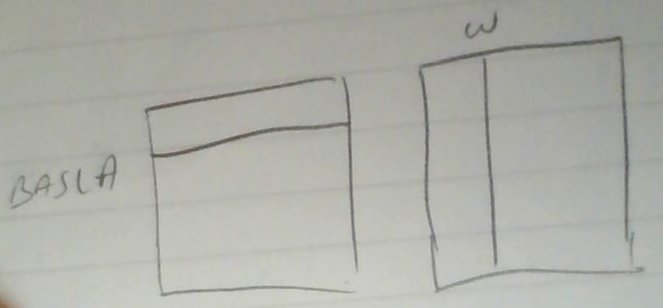
\includegraphics[height=4cm]{crf_3.jpg}

Bu ifadenin sol taraftaki $M_1$ içinde $\textrm{BAŞLA}$ satırını sağ taraftaki $M_2$
$w$ kolonu ile çarptığını düşünebiliriz.

$$M_{12}(\textrm{BAŞLA},w) = \sum_v M_1(\textrm{BAŞLA}, v)M_2(v,w)  $$

$$ = \sum_v \exp [g_1(\textrm{BAŞLA},v) + g_2(v,w)] $$

Bu istediğimiz gibi bir ifadeye dönüşmeye başladı, çünkü hatırlarsak, (5)'e
benzeyen bir şeyleri elde etmeye uğraşıyoruz. Gerçi üstteki ifade tüm $y$
değerleri için değil, tek bir $v$ için, ama yine de uygun, üstteki $v$
yerine $y_1$ dersek belki daha uygun olur,

$$ = \sum_{y_1} \exp [g_1(\textrm{BAŞLA},y_1) + g_2(y_1,w)] $$

Üçlü bir çarpma görelim: $M_{123}$. 

$$ M_{123} = \sum_{y_2} M_{12}(\textrm{BAŞLA}, y_2)M_3(y_2,w)  $$

$$ = \sum_{y_2} [ \sum_{y_1}\exp [g_1(\textrm{BAŞLA},y_1) + g_2(y_1y_2) ] 
\exp g_3(y_2,w) ]
$$

$$ \sum_{y_1,y_2} \exp [g_1(\textrm{BAŞLA},y_1) + g_2(y_1y_2) + g_3(y_2,v)]  $$

Yani üç matrisi birbiriyle çarparak $y_1,y_2$ üzerinden toplam almış
oluyorum. Ve böyle devam edersem, yani tüm matrisleri birbiriyle çarparsam
ve $\textrm{BAŞLA}, \textrm{BİTİŞ}$ değerlerine bakarsam, 

$$ 
M_{123...n+1} (\textrm{BAŞLA}, \textrm{BİTİŞ}) =  
$$
$$
\sum_{y_1,...,y_n}  \exp [
(g_1(\textrm{BAŞLA},y_1) + g_2(y_1,y_2) + g_3(y_2,y_3) + ... + g_{n+1}
(y_n, \textrm{BİTİŞ} )
]
$$

Bu ifade parçalara ayırma (partition) fonsiyonu için tam ihtiyacım olan
şey. Daha önce Viterbi algoritmasından bahsettik, hatta bu algoritma
dinamik programlama kategorisine girer dedik, üstteki algoritma dinamik
programlama bile sayılmaz, aslında bir matris çarpımı sadece. Daha genel
olarak üstteki algoritma ileri-geri (forward-backward) algoritmasının bir
türevi, bu algoritmalar bildiğimiz gibi HMM'lerde sıkça kullanılıyorlar.

Bu iki algoritma CRF'ler için gerekli. Şimdi CRF'leri nasıl eğiteceğimizi
görelim. 

Eğitim

Maksimizasyon için rasgele gradyan çıkışı kullanacağız. 

$$ 
p(y|x;w) = \frac{\exp \sum_j w_j F_j(x,y)  }{Z(x;w)}
$$

Gradyan çıkışı için üstteki formülün türevini alabilmeliyiz. Önce
$\log$'unu almak lazım, çünkü $\partial / \partial w_j \log p$ hesabı
gerekli, üsttekinin $\log$'u ise bölümün $\log$'u eksi bölenin $\log$'u.

$$
 \frac{\partial}{\partial w_j} \log p
=
\frac{\partial}{\partial w_j} [ \sum_j w_j F_j(x,y)] -
\frac{\partial}{\partial w_j} \log Z(x;w)
 $$

Türevin eksi öncesi ilk bölümü çok basit, $w_j$ ve toplam yokolacak (tüm
$j$'lerin toplamı yokoldu, çünkü türev ``tek'' bir $j$ değeri ile
ilgileniyor, diğerleri sıfır oluyor)


$$ 
= F_j(x,y) -
\frac{\partial}{\partial w_j} \log Z(x;w)
$$

Eksiden sonraki kısım çok zarif bir sonuca dönüşecek, birazdan göreceğiz. 

$$ 
\frac{\partial}{\partial w_j} \log Z(x;w) = 
\frac{1}{Z} \frac{\partial}{\partial w_j} Z 
$$

Türevi toplam içine taşıyoruz, 

$$ 
= \frac{1}{Z} \sum_{y'} \frac{\partial}{\partial w_j} [
\exp [ \sum_{j'} w_j' F_{j'}(x,y') ] ] 
$$

$$  
= \frac{1}{Z}\sum_{y'} 
\bigg[
\exp [ \sum_{j'} w_{j'} F_{j'}(x,y') ] F_j(x,y')
\bigg]
$$

$$ 
= \sum_{y'} F_j (x,y')
\frac{
\exp [ \sum_{j'} w_{j'} F_{j'}(x,y') ]
}
{Z}
$$ 

Şimdi ilginç kısma geldik, üstteki kesirli kısım $p(y' | x;w)$ değerine
eşittir. 

$$ = \sum_{y'} F_j (x,y') p(y' | x;w)$$ 

İlginç durum burada ortaya çıkıyor, çünkü üstteki aynı zamanda bir beklenti
(expectation) tanımı değil mi? Tüm $F_j$ değerlerini o değerlerin
olasılıkları ile çarpıp toplarsak bir beklenti elde etmez miyiz? Evet. O
zaman beklenti tanımını kullanabiliriz,

$$\frac{\partial}{\partial w_j} \log p = F_j(x,y) - E[F_j(x,y') ] $$

ki $y'$ şöyle bir dağılımı takip ediyor, 

$$ y' \sim p(y'|x;w) $$

Soru: $\frac{\partial}{\partial w_j} \log p = ?$ Yani bu türev ne zaman 
sıfıra eşittir? 

Cevap: Türevin açılımına bakınca mesela, $F_j=0$ olunca mı? Hayır, çünkü OF
sıfır olsa bile beklenti kısmı sıfır olmayabilir. O zaman şöyle söylemek
gerekir, eğer tüm $y'$ için $F_j(x,y') - 0$ ise, o zaman türev sıfır olur. 

Çoğunlukla $F_j(x,y) = a(x)I(y=v)$. Hatırlarsak bu yöntem bir özelliği (ki
$(a(x)$ ile temsil ediliyor), her mümkün $v$ değeri için bir OF'ye
çevirmenin yolu idi (tek $x$'e bağlı OF olamaz).

O zaman şunu da söyleyebiliriz, eğer $a(x) = 0$ ise, her $y$ için $F_j(x,y)
= 0$ demektir. 

Bu bilginin faydası şudur, veride seyreklik var ise, lojistik regresyon
bunları atlamayı bilir. Demek ki aynı şekilde koşulsal lineer modeller de
bu özellikleri atlayabilir. Eğer bir özellik $a(x)=0$ ise, o özellik
ağırlık güncellemesi (weight update) sırasında atlanır. 

Algoritma \verb!train_crf!
\begin{itemize}
   \item Her eğitim noktası $x,y$ için
   \begin{itemize}
      \item $j$ için
     \begin{itemize}
       \item $E[F_j(x,y')]$ hesapla (buna sadece $E$ diyelim) 
       \item Güncelle: $w_j := w_j + \lambda[F_j(x,y) - E]$
    \end{itemize}
   \end{itemize}
\end{itemize}

Bu hesabın en pahalı kısmı neresi? Beklenti hesabı. Bu beklentileri
hesaplanması için daha önce verdiğimiz matris çarpımı yöntemine benzer bir
yöntem kullanmak gerekiyor (burada vermeyeceğiz, arama motorunda Rahul
Gupta üzerinden arayabilirsiniz, bu kişi bu konuyu anlatıyor).

Kaynak

[1] Elkan, {\em Log-linear Models and Conditional Random Fields}, 
    \url{http://videolectures.net/cikm08_elkan_llmacrf}

\end{document}



